\chapter{Die Synthese-Pipeline}
\label{kap:pipeline}

Dieses Kapitel dokumentiert die Pipeline, die aus neun Objektausschnitten und
sieben Hintergrundaufnahmen den vollständigen Trainingsdatensatz erzeugt. Die in
Tabelle~\ref{tab:parameter} genannten Anteile sind keine konfigurierten
Sollwerte, sondern \emph{gemessene} Ist-Werte aus dem Erzeugungsbericht
\code{synth/train/generation\_report.json} über 6000 Bilder mit 173\,100
gerenderten Instanzen und 136\,384 gelabelten Objekten.

\section{Leitprinzip und Arbeitsteilung}
\label{sec:leitprinzip}

\absatz{Leitprinzip.} Die Pipeline verfolgt genau ein Ziel: \emph{jede Abkürzung
schließen, über die ein CNN \enquote{hier wurde etwas eingeklebt} statt
\enquote{hier ist ein Rohrende} lernen könnte.} Wie in
Abschnitt~\ref{sec:shortcut} begründet, ist bei Copy-Paste-Synthese nicht zu
wenig Variation die dominante Fehlerquelle, sondern der systematische
Unterschied zwischen eingefügten und originalen Pixeln.

\absatz{Arbeitsteilung.} Aus Anforderung~A1 folgt, wo eine Transformation
ausgeführt wird: Der \textbf{Generator} übernimmt alles, was \emph{pro Instanz}
wirkt und die Box aus der transformierten Alphamaske exakt neu bestimmt --
Rotation über den vollen Kreis, Ovalisierung, Delle, Perspektive, Photometrie,
Verdeckung, Sichtbarkeitsrechnung. Die \textbf{Trainingszeit-Augmentierung}
übernimmt alles, was \emph{bildweit} wirkt und Boxen nicht verfälscht -- Mosaic,
Skalierung, Translation, Spiegelung, HSV-Variation. Daraus folgt zwingend, dass
im Training \code{degrees}, \code{shear} und \code{perspective} auf~0 stehen: Sie
blähen achsparallele Boxen auf (Abschnitt~\ref{sec:boxrotation}). Die
entsprechenden Invarianzen werden also nicht \emph{weggelassen}, sondern an
anderer Stelle und label-exakt erzeugt.

\begin{figure}[htbp]
\centering
\begin{tikzpicture}[
  box/.style={draw,rounded corners=2pt,align=center,font=\scriptsize,
              text width=1.8cm,minimum height=8mm,inner sep=2.5pt,fill=blue!8},
  stage/.style={draw,rounded corners=2pt,align=center,font=\scriptsize,
              text width=1.8cm,minimum height=9mm,inner sep=2.5pt,fill=orange!18},
  erg/.style={draw,rounded corners=2pt,align=center,font=\scriptsize,
              text width=2.0cm,minimum height=9mm,inner sep=2.5pt,fill=green!12},
  ar/.style={-{Latex[length=1.8mm]},semithick,gray!60!black}]
  \node[box]   (cut)   at (0,1.15)  {9 Objekt-\\ausschnitte};
  \node[box]   (bg)    at (0,-1.15) {7 Hintergrund-\\aufnahmen};
  \node[stage] (mat)   at (2.8,1.15) {\textbf{Stufe 1}\\Matting};
  \node[stage] (occ)   at (2.8,-1.15){\textbf{Stufe 2}\\Okkluder};
  \node[box]   (masks) at (5.5,1.15) {9 Alphamasken\\(1,1\,px Kante)};
  \node[box]   (bars)  at (5.5,-1.15){56 echte\\Rohrschäfte};
  \node[stage] (syn)   at (8.3,0)    {\textbf{Stufe 3}\\Synthese\\T1--T9};
  \node[erg]   (ds)    at (11.1,0)   {6000 Bilder\\136\,384 Labels};
  \draw[ar] (cut) -- (mat);   \draw[ar] (bg)  -- (occ);
  \draw[ar] (mat) -- (masks); \draw[ar] (occ) -- (bars);
  \draw[ar] (masks) -- (syn); \draw[ar] (bars)  -- (syn);
  \draw[ar] (bg.south) -- ++(0,-0.65) -| (syn.south);
  \draw[ar] (syn) -- (ds);
  \node[font=\scriptsize,gray!50!black,fill=white,inner sep=1.5pt]
        at (4.0,-2.2) {Hintergründe zusätzlich direkt};
\end{tikzpicture}
\caption[Aufbau der Pipeline]{Aufbau der Pipeline. Die Hintergrundaufnahmen
werden zweifach genutzt: als Quelle der Okkluder-Bibliothek und unmittelbar als
Bildhintergrund und Fremdkörperquelle.}
\label{abb:pipeline}
\end{figure}

\section{Vorstufen: Freistellen und Okkluder-Bibliothek}
\label{sec:matting}

\absatz{Stufe 1 -- Matting.} Nach Befund~1 sind alle neun Ausschnitte
rechteckig; direktes Einkopieren erzeugte Signatur~S1. Das Freistellen erfolgt
dreistufig über ein Ellipsenmodell $(c_x, c_y, r_x, r_y, \theta)$: manuelle
Startwerte aus einer 14-fach vergrößerten Rasteransicht, numerische Verfeinerung
per Coordinate Descent auf der radialen Kantenenergie
$I(\text{innen}) - I(\text{außen})$ eines sechsfach upgesampelten Bildes, und
eine Außenkantenkorrektur. Letztere ist nötig, weil die Optimierung
konstruktionsbedingt auf dem \emph{Grat} des hellen Kranzes konvergiert und nicht
auf seiner Außenkante; ein mittleres Radialprofil bestimmt daher den Radius, bei
dem die Helligkeit auf 25\,\% der Kantenamplitude über Hintergrundniveau
abgefallen ist.

Die Wahl von 25\,\% statt des klassischen Halbwertspunkts
\parencite{gonzalez2018} verschiebt die Maskengrenze bewusst nach außen, weil die
Kosten asymmetrisch sind: Der helle Kranz ist das \emph{diskriminative} Merkmal
-- ihn anzuschneiden entfernt Information, die das Netz braucht --, während ein
etwa 1\px{} breiter Hintergrundsaum durch Feathering und Farbangleich ohnehin
kaschiert wird. Die Aufweitung ist hart auf $[1{,}02;\,1{,}10]$ gedeckelt: Bei
acht der neun Ausschnitte liegt der ermittelte Faktor bei 1,02--1,05, nur der
kontrastarme neunte liefe sonst auf 1,19 und die Maske würde Hintergrund
aufsaugen. Ergebnis sind weiche Alphamasken mit rund 1,1\px{} Übergangsbreite --
Absicht und nicht Toleranz, denn ein 25\px{} großes Objekt hat in einer echten
Aufnahme nie eine pixelharte Silhouette.

\absatz{Stufe 2 -- Okkluder.} Ein synthetisch \emph{gemalter} Balken hätte andere
Textur-, Rausch- und Glanzstatistik als der Rest des Bildes -- das Netz könnte
\enquote{Objekt liegt neben künstlichem Balken} lernen, also eine Abkürzung der
Klasse S2--S4. Die vier Clean Plates sind dagegen Wände aus Rohrschäften
desselben Materials, derselben Kamera und derselben Beleuchtung. Aus ihnen werden
Okkluder gewonnen: dominante Rohrrichtung über den Struktur-Tensor
\parencite{jaehne2005} und Drehung des Bildes (gemessen $+0{,}9$, $-1{,}6$,
$+0{,}9$, $+6{,}6$ Grad), Hochpassfilterung des Zeilenmittelprofils zur
Bestimmung der Rohrachsen -- ihr Abstand ist der Rohrdurchmesser
(16/18/21/20\px, dieselben Werte, die den Maßstab verankern) --, Ausschneiden
eines Streifens je Achse und eine weiche Kapselmaske mit 1,6\px{} Feder.
Ergebnis sind 56 Rohrschäfte mit echter zylindrischer Schattierung und echtem
Glanzlicht; sie dienen als Schaft \emph{hinter} jeder Stirnfläche
(Tabelle~\ref{tab:parameter}, T5) und als Okkluder \emph{vor} dem Stapel.

\section{Stufe 3 -- Bildsynthese}
\label{sec:synthese}

Die Leinwand ist $1024\times1024$ Pixel groß und damit identisch zur
Trainingsauflösung. Das ist eine bewusste Entscheidung nach Anforderung~A2: Die
synthetischen Bilder durchlaufen im Training \emph{keine} Größenänderung, die
kalibrierte Objektgrößenverteilung bleibt exakt erhalten.
Tabelle~\ref{tab:stufen} gibt den Überblick, Tabelle~\ref{tab:parameter} im
Anhang dokumentiert alle 36 Transformationen einzeln mit Parameterbereich,
gemessenem Ist-Anteil und Begründung. Die folgenden Abschnitte begründen die fünf
Stellen, an denen die Modellierung über eine Parameterwahl hinausgeht.

\begin{table}[htbp]
\centering
\caption[Überblick der Synthesestufen]{Überblick der neun Synthesestufen.
Die vollständige Dokumentation aller 36 Transformationen mit Parameterbereich,
gemessenem Ist-Anteil und Begründung steht in Tabelle~\ref{tab:parameter} im
Anhang.}
\label{tab:stufen}
\footnotesize
\begin{tabularx}{\textwidth}{@{}llX@{}}
\toprule
\textbf{Stufe} & \textbf{Anz.} & \textbf{Inhalt und zentrale Parameter} \\
\midrule
T1 Hintergrund & 7 &
Clean Plate (80\,\%), Zoom an Rohr-\Oe{} gekoppelt, Zufallsausschnitt,
Reflect-Padding, Spiegelungen (50/15\,\%), Kleinrotation $\pm6^\circ$ \\
T2 Instanzgeometrie & 5 &
Rotation $0$--$360^\circ$ (100\,\%), Skalierung 12--44\px, Ovalisierung
(57\,\%), Delle (18\,\%), Perspektive $\pm9\,\%$ (30\,\%) \\
T3 Photometrie & 8 &
Helligkeit, Gamma, HSV, Farbangleich (85\,\%), Unschärfe- und Rauschangleich,
Kantenweichzeichnung, Schlagschatten (49\,\%) \\
T4 Layout & 2 &
gescherte Gitterpackung, 1--3 Cluster; abgedunkelte Mulde \\
T5 Rohrschaft & 4 &
echter Schaft hinter 88\,\% der Instanzen, parallele Richtung $\pm11^\circ$,
Helligkeitsangleich, Tiefenmodell 75/25 \\
T6 Okklusion & 2 &
quer liegende Rohrstangen (58\,\% der Bilder), Fremdkörper (32\,\%) \\
T7 Sichtbarkeit & -- &
exakte Rechnung und Labelregeln, Abschnitt~\ref{sec:sichtbarkeit} \\
T8 globale Bildstufe & 7 &
Helligkeit/Kontrast, HSV, Defokus, Bewegungsunschärfe, Rauschen,
Vignettierung, JPEG-Requantisierung (85\,\%) \\
T9 Negativbilder & 1 &
9,7\,\% der Bilder ohne jedes Objekt \\
\bottomrule
\end{tabularx}
\end{table}

\begin{figure}[htbp]
\centering
\begin{subfigure}{0.315\textwidth}
  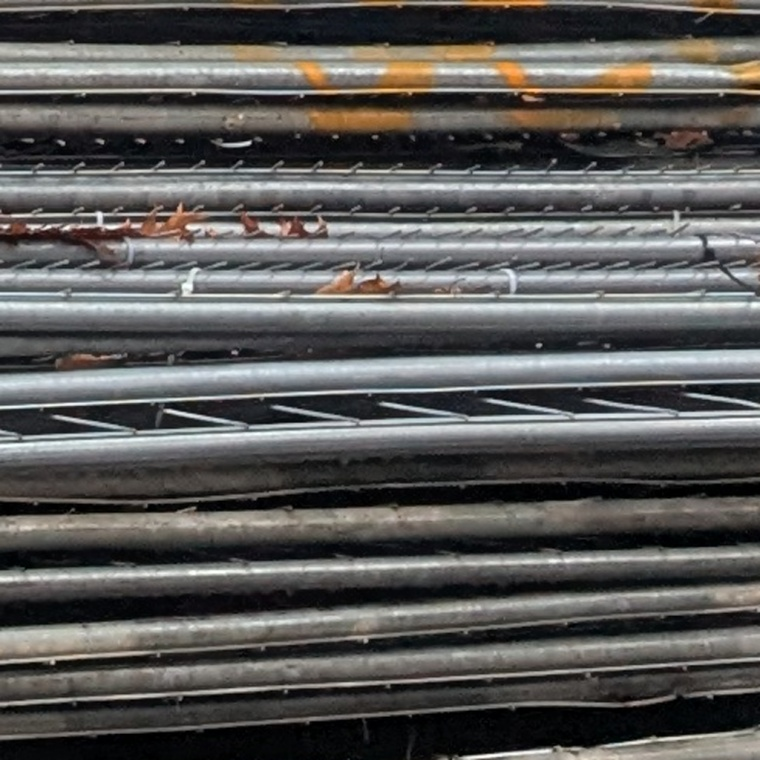
\includegraphics[width=\textwidth]{abbildungen/stufe_T1_hintergrund.jpg}
  \caption{T1 Hintergrund}
\end{subfigure}\hfill
\begin{subfigure}{0.315\textwidth}
  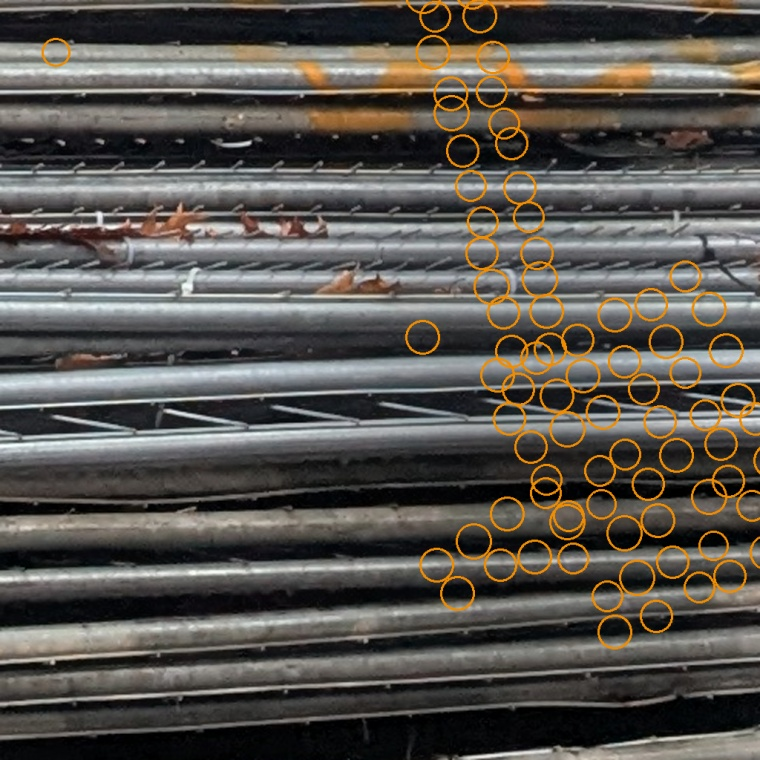
\includegraphics[width=\textwidth]{abbildungen/stufe_T4_layout.jpg}
  \caption{T4 Layout}
\end{subfigure}\hfill
\begin{subfigure}{0.315\textwidth}
  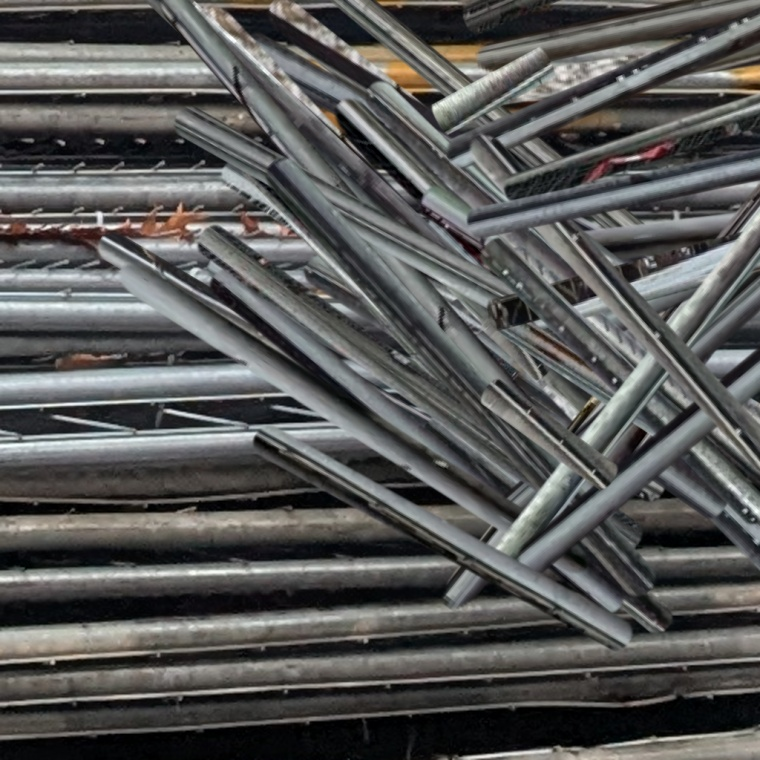
\includegraphics[width=\textwidth]{abbildungen/stufe_T5_schaft.jpg}
  \caption{T5 Rohrschaft}
\end{subfigure}

\vspace{4pt}
\begin{subfigure}{0.315\textwidth}
  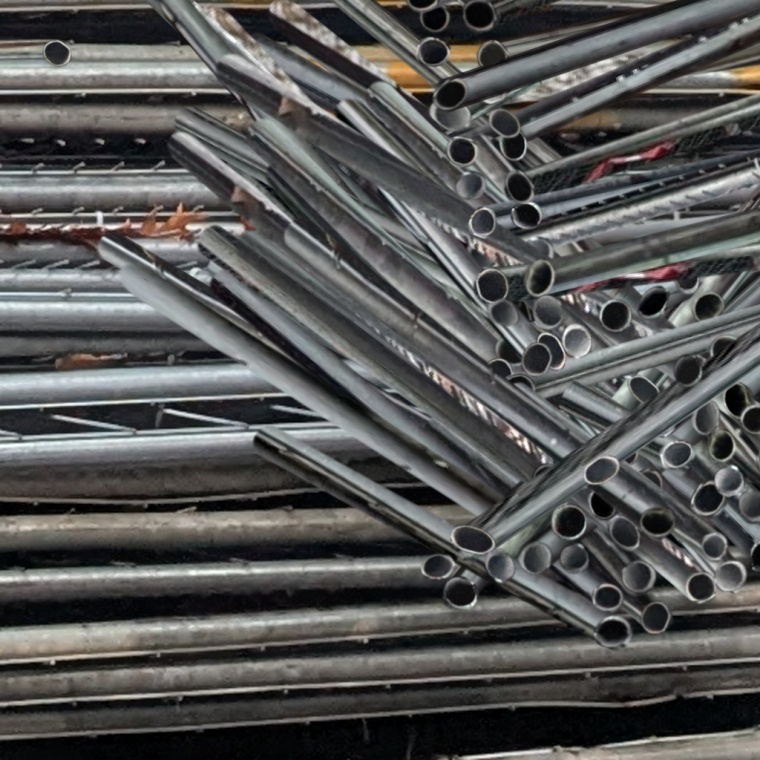
\includegraphics[width=\textwidth]{abbildungen/stufe_T2T3_instanzen.jpg}
  \caption{T2/T3 Instanzen}
\end{subfigure}\hfill
\begin{subfigure}{0.315\textwidth}
  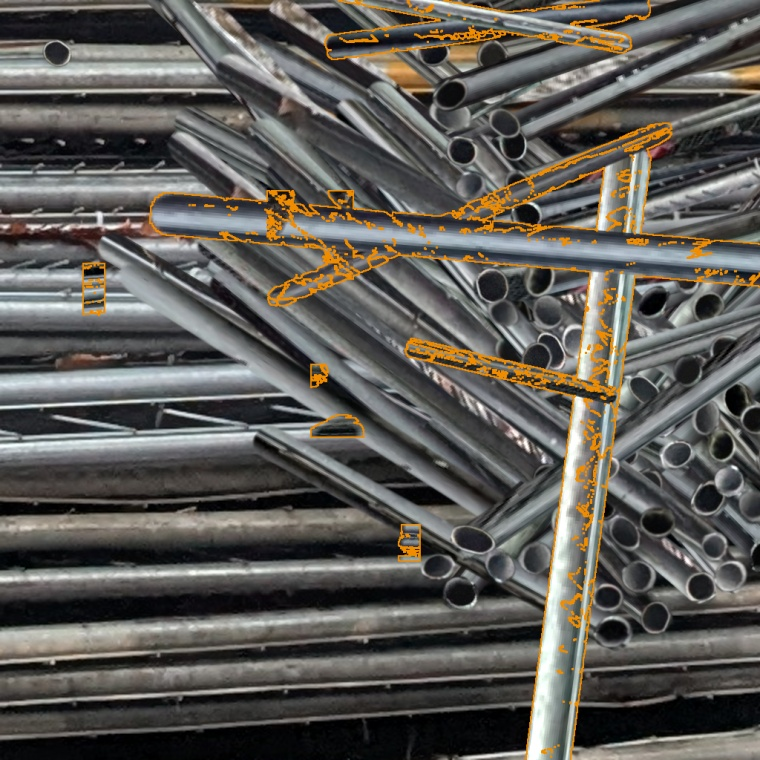
\includegraphics[width=\textwidth]{abbildungen/stufe_T6_okklusion.jpg}
  \caption{T6 Okklusion}
\end{subfigure}\hfill
\begin{subfigure}{0.315\textwidth}
  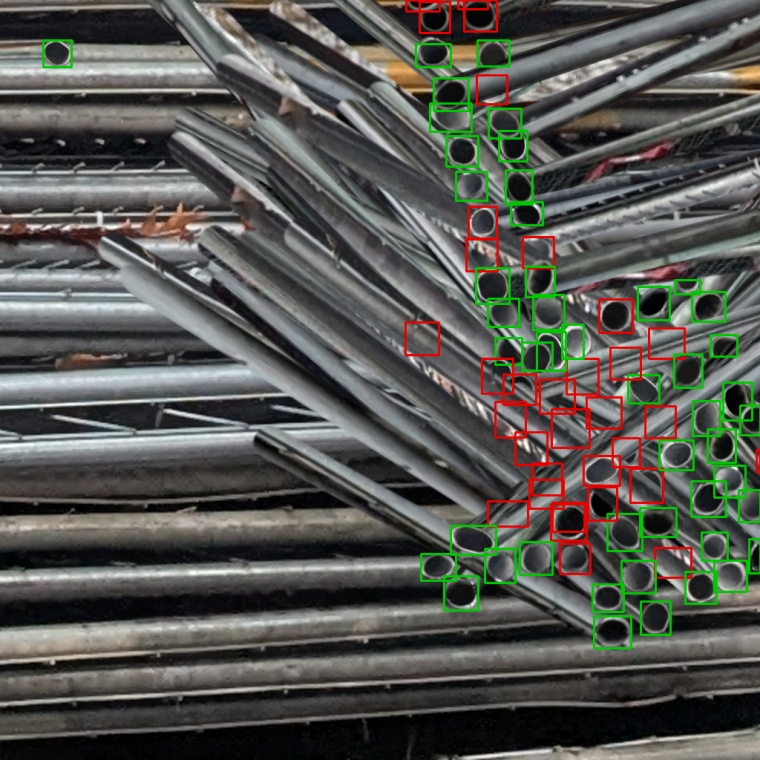
\includegraphics[width=\textwidth]{abbildungen/stufe_T7_sichtbarkeit.jpg}
  \caption{T7 Sichtbarkeit}
\end{subfigure}
\caption[Aufbau eines synthetischen Bildes]{Aufbau eines synthetischen Bildes,
Stufe für Stufe am selben Bild. (a)~Der gewählte Clean Plate nach Zoom,
Ausschnitt und Spiegelung. (b)~Die gezogenen Objektzentren des Layoutmodells
(orange), dazu zwei abgedunkelte Mulden. (c)~Die Rohrschäfte, in paralleler
Richtung und zu 75\,\% ganz hinten gemalt. (d)~Die Stirnflächen mit
Instanzgeometrie und Photometrie -- 82 Instanzen. (e)~Was die Okklusionsstufe
hinzufügt, orange umrandet: sechs quer liegende Stangen und Fremdkörper.
(f)~Das Urteil der Sichtbarkeitsrechnung: grün die 48 vergebenen Labels, rot
die 33 verworfenen Instanzen. Die Einzelstufen T2, T3, T8 und T9 sind in den
Abbildungen~\ref{abb:stufendetail} und~\ref{abb:stufenglobal} im Anhang
vergrößert dargestellt. Zur Lesbarkeit ist ein Bild am oberen Ende des
Größenbereichs gewählt (Basisdurchmesser 44\px{} statt des Medians von
22,5\px) und mit überdurchschnittlicher Verdeckung;
Abbildung~\ref{abb:synthbeispiele} zeigt typische Bilder. Erzeugt mit
\code{paper/tools/fig\_stufen.py}, Seed~302.}
\label{abb:stufen}
\end{figure}

\subsection{Fünf Modellierungsentscheidungen}

\absatz{Maßstabskopplung.} Der Zoomfaktor $z$ wird so gezogen, dass der
Basisdurchmesser im Zielbereich $[12, 44]$\px{} liegt:
\begin{equation}
z \sim \mathcal{U}\!\left[\max\!\left(0{,}55,\;
\tfrac{d_{\min}}{d_{\text{Rohr}}}\right),\;
\min\!\left(2{,}20,\;\tfrac{d_{\max}}{d_{\text{Rohr}}}\right)\right],
\qquad d_{\text{Basis}} = d_{\text{Rohr}} \cdot z .
\label{eq:zoom}
\end{equation}
Objektgröße und Hintergrundmaßstab sind damit \emph{nicht} unabhängig gezogen --
der Kern von Anforderung~A3.

\begin{figure}[htbp]
\centering
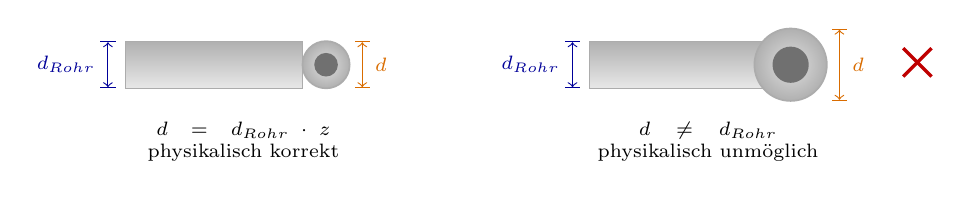
\begin{tikzpicture}
\foreach \r/\ok/\sh/\lab in {%
   0.30/1/0/{$d = d_{\text{Rohr}}\cdot z$\\physikalisch korrekt},
   0.46/0/5.9/{$d \neq d_{\text{Rohr}}$\\physikalisch unmöglich}}{
  \begin{scope}[shift={(\sh,0)}]
    \shade[top color=gray!62,bottom color=gray!18] (0,0.28) rectangle (2.25,0.88);
    \draw[gray!65,thin] (0,0.28) rectangle (2.25,0.88);
    \shade[inner color=gray!25,outer color=gray!62] (2.55,0.58) circle (\r);
    \draw[gray!65,semithick] (2.55,0.58) circle (\r);
    \fill[gray!88!black] (2.55,0.58) circle ({\r*0.5});
    \draw[|<->|,thin,blue!60!black] (-0.22,0.28) -- (-0.22,0.88);
    \node[font=\scriptsize,anchor=east,blue!60!black] at (-0.26,0.58)
         {$d_{\text{Rohr}}$};
    \draw[|<->|,thin,orange!85!black] ({2.55+\r+0.16},{0.58-\r})
          -- ({2.55+\r+0.16},{0.58+\r});
    \node[font=\scriptsize,anchor=west,orange!85!black]
         at ({2.55+\r+0.20},0.58) {$d$};
    \ifnum\ok=0
      \draw[red!75!black,very thick] (3.98,0.79) -- (4.34,0.43);
      \draw[red!75!black,very thick] (3.98,0.43) -- (4.34,0.79);
    \fi
    \node[font=\scriptsize,anchor=north,align=center,text width=5.2cm]
         at (1.5,-0.02) {\lab};
  \end{scope}}
\end{tikzpicture}
\caption[Maßstabskopplung]{Die Maßstabskopplung aus
Gleichung~\eqref{eq:zoom}. Links: Die Stirnfläche hat denselben Durchmesser wie
der Schaft, an dem sie sitzt -- es ist dasselbe Rohr. Rechts: Würden Zoom und
Objektgröße unabhängig gezogen, entstünde ein Missverhältnis, das real nicht
vorkommt und dem Netz eine falsche Kontext-Größen-Relation antrainierte.}
\label{abb:zoomkopplung}
\end{figure}

\absatz{Skalierung und Ovalisierung} werden in einem Schritt ausgeführt. Mit
Quelldurchmesser $d_{\text{src}}$, Zieldurchmesser $d$ und gezogenem
Achsverhältnis $\rho$ gilt
\begin{equation}
s_x = \frac{d}{d_{\text{src}}\sqrt{\rho}}, \qquad
s_y = \frac{d\,\sqrt{\rho}}{d_{\text{src}}},
\qquad\text{also}\quad \sqrt{s_x s_y}\, d_{\text{src}} = d .
\label{eq:oval}
\end{equation}
Der geometrische Mittelwert bleibt erhalten -- notwendig, damit die Ovalisierung
die kalibrierte Größenverteilung nicht verschiebt, denn die Realmessung verwendet
mit $\sqrt{\text{Fläche}}$ genau dieses Maß.

\begin{figure}[htbp]
\centering
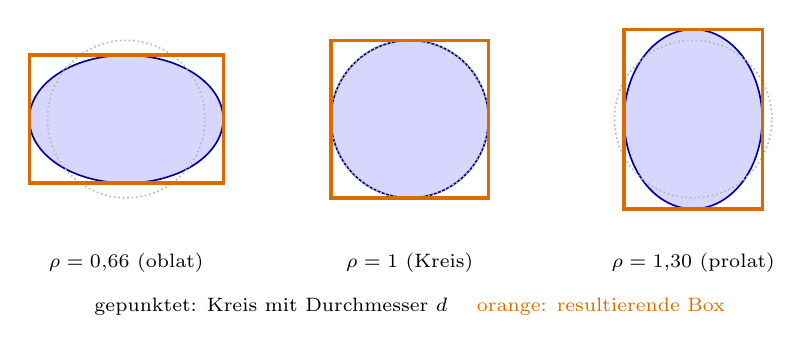
\begin{tikzpicture}
\foreach \rr/\lab/\sh in {%
   0.66/{$\rho = 0{,}66$ (oblat)}/0,
   1.00/{$\rho = 1$ (Kreis)}/3.6,
   1.30/{$\rho = 1{,}30$ (prolat)}/7.2}{
  \begin{scope}[shift={(\sh,0)}]
    \pgfmathsetmacro{\ax}{1/sqrt(\rr)}
    \pgfmathsetmacro{\by}{sqrt(\rr)}
    \fill[blue!16] (0,0) ellipse ({\ax} and {\by});
    \draw[blue!60!black,semithick] (0,0) ellipse ({\ax} and {\by});
    \draw[gray!55,densely dotted,semithick] (0,0) circle (1);
    \draw[very thick,orange!85!black] ({-\ax},{-\by}) rectangle ({\ax},{\by});
    \node[font=\scriptsize,anchor=north,align=center] at (0,-1.58) {\lab};
  \end{scope}}
\node[font=\scriptsize,anchor=north,align=center] at (3.6,-2.15)
     {gepunktet: Kreis mit Durchmesser $d$ \quad
      \textcolor{orange!85!black}{orange: resultierende Box}};
\end{tikzpicture}
\caption[Ovalisierung]{Ovalisierung nach Gleichung~\eqref{eq:oval}. Alle drei
Ellipsen haben dieselbe Fläche wie der gepunktete Kreis mit Durchmesser $d$, weil
in der Breite mit $1/\sqrt{\rho}$ und in der Höhe mit $\sqrt{\rho}$
skaliert wird: Der geometrische Mittelwert $\sqrt{s_x s_y}\,d_{\text{src}} = d$
bleibt erhalten. Die daraus abgeleitete Box (orange) ändert sich dagegen -- und
genau deren Seitenverhältnis ist die an den Realdaten gemessene Größe.}
\label{abb:ovalisierung}
\end{figure}

\absatz{Farbangleich.} Ein \emph{partieller} Statistiktransfer im Stil von
\textcite{reinhard2001}: Mit Mittelwert und Streuung der Objektpixel
($\mu_i, \sigma_i$) und des lokalen Hintergrunds ($\mu_b, \sigma_b$) gilt je
Farbkanal
\begin{equation}
c' = \mu_i + k\,(c - \mu_i) + \alpha_\mu\,(\mu_b - \mu_i),
\quad
k = 1 + \alpha_\sigma\!\left(\operatorname{clip}\!\left(
\tfrac{\sigma_b}{\sigma_i},\, 0{,}6,\, 1{,}6\right) - 1\right)
\label{eq:harmonize}
\end{equation}
mit $\alpha_\mu \sim \mathcal{U}[0{,}10;\,0{,}45]$ und
$\alpha_\sigma \sim \mathcal{U}[0;\,0{,}35]$. Für
$\alpha_\mu = \alpha_\sigma = 1$ ginge das in den vollständigen
Reinhard-Transfer über -- genau das ist \emph{nicht} gewollt: Ein vollständiger
Angleich ebnete den intrinsischen Albedo-Unterschied zwischen Bohrung und Kranz
ein und zerstörte damit das Objekt. Modelliert wird ausschließlich die
Beleuchtungs- und Weißabgleichdifferenz, nicht die Objektfarbe.

\begin{figure}[htbp]
\centering
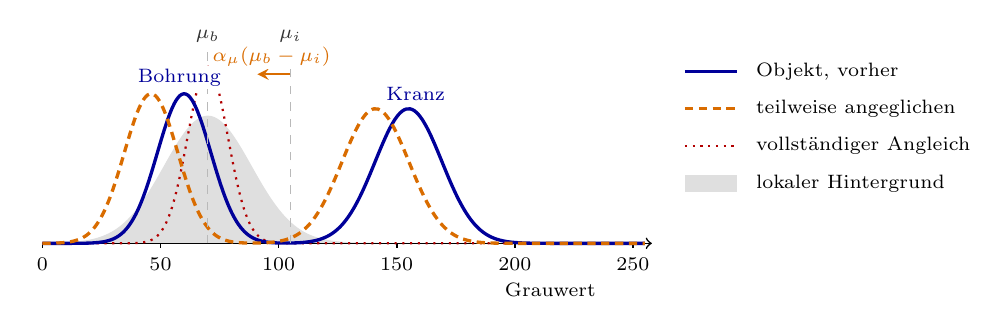
\begin{tikzpicture}[x=0.030cm,y=1.9cm]
  \draw[gray!25,fill=gray!25,smooth]
    plot[domain=0:255,samples=110] (\x, {0.85*exp(-((\x-70)/26)^2)})
    -- (255,0) -- (0,0) -- cycle;
  \draw[->,semithick] (0,0) -- (258,0);
  \node[font=\scriptsize,anchor=north] at (215,-0.20) {Grauwert};
  \foreach \g in {0,50,100,150,200,250}
    \draw[semithick] (\g,0) -- (\g,-0.030) node[below,font=\scriptsize] {\g};
  \draw[red!70!black,thick,dotted,smooth]
    plot[domain=0:255,samples=150] (\x, {1.18*exp(-((\x-70)/12)^2)});
  \draw[very thick,blue!60!black,smooth]
    plot[domain=0:255,samples=150]
    (\x, {exp(-((\x-60)/16)^2) + 0.9*exp(-((\x-155)/20)^2)});
  \draw[very thick,orange!85!black,densely dashed,smooth]
    plot[domain=0:255,samples=150]
    (\x, {exp(-((\x-46)/16)^2) + 0.9*exp(-((\x-141)/20)^2)});
  \draw[dashed,gray!55] (70,0) -- (70,1.34);
  \node[font=\scriptsize,gray!40!black,anchor=south,fill=white,inner sep=1pt]
       at (70,1.32) {$\mu_b$};
  \draw[dashed,gray!55] (105,0) -- (105,1.34);
  \node[font=\scriptsize,gray!40!black,anchor=south,fill=white,inner sep=1pt]
       at (105,1.32) {$\mu_i$};
  \draw[->,>=stealth,orange!85!black,thick] (105,1.13) -- (91,1.13);
  \node[font=\scriptsize,orange!85!black,anchor=south,inner sep=1pt,
        fill=white] at (97,1.16) {$\alpha_\mu(\mu_b - \mu_i)$};
  \node[font=\scriptsize,blue!60!black,anchor=south,fill=white,inner sep=1pt]
       at (58,1.03) {Bohrung};
  \node[font=\scriptsize,blue!60!black,anchor=south,fill=white,inner sep=1pt]
       at (158,0.93) {Kranz};
  % Legende rechts neben der Achse
  \begin{scope}[shift={(272,0)}]
    \draw[very thick,blue!60!black] (0,1.15) -- (22,1.15);
    \node[font=\scriptsize,anchor=west] at (26,1.15) {Objekt, vorher};
    \draw[very thick,orange!85!black,densely dashed] (0,0.90) -- (22,0.90);
    \node[font=\scriptsize,anchor=west] at (26,0.90) {teilweise angeglichen};
    \draw[thick,red!70!black,dotted] (0,0.65) -- (22,0.65);
    \node[font=\scriptsize,anchor=west] at (26,0.65) {vollständiger Angleich};
    \fill[gray!25] (0,0.34) rectangle (22,0.46);
    \node[font=\scriptsize,anchor=west] at (26,0.40) {lokaler Hintergrund};
  \end{scope}
\end{tikzpicture}
\caption[Partieller Farbangleich]{Partieller Farbangleich nach
Gleichung~\eqref{eq:harmonize}. Die Grauwertverteilung des Objekts ist
zweigipfelig: dunkle Bohrung und heller Kranz. Der Angleich verschiebt sie um
$\alpha_\mu(\mu_b - \mu_i)$ in Richtung des lokalen Hintergrunds, hält die
beiden Gipfel aber auseinander. Ein vollständiger Angleich
($\alpha_\mu = \alpha_\sigma = 1$, gepunktet) zöge sie auf die
Hintergrundverteilung zusammen und zerstörte damit den Albedo-Unterschied, der
das Objekt überhaupt erkennbar macht.}
\label{abb:farbangleich}
\end{figure}

\absatz{Rauschschätzung.} Das lokale Rauschniveau wird als Streuung eines
Hochpassrests geschätzt \parencite[vgl.][]{immerkaer1996} -- mit einem
Medianfilter als Tiefpass, weil er Kanten weniger verschmiert:
\begin{equation}
\hat{\sigma} = \operatorname{std}\!\big(g - \operatorname{median}_{3\times3}(g)\big),
\quad
\sigma_{\text{Rausch}} = \max\!\big(0{,}5,\; \hat{\sigma} \cdot
\mathcal{U}[0{,}5;\,1{,}25]\big).
\label{eq:noise}
\end{equation}

\iffalse

\begin{figure}[htbp]
\centering
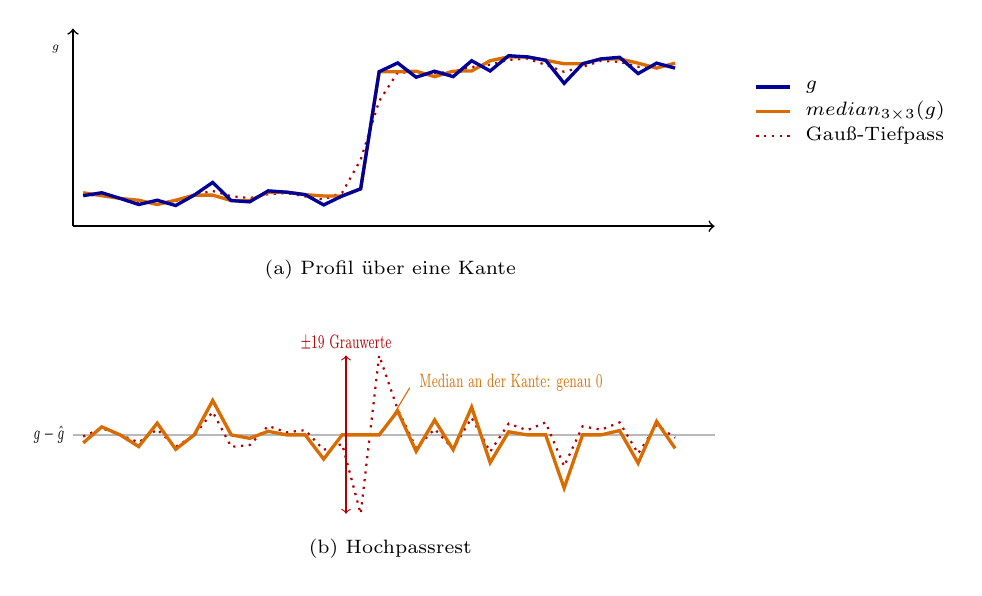
\begin{tikzpicture}
\begin{scope}[xscale=1.62,yscale=1.55]
  \draw[->,semithick] (-0.08,0) -- (4.95,0);
  \draw[->,semithick] (-0.08,0) -- (-0.08,1.62);
  \node[font=\scriptsize,anchor=east,xscale=0.617,yscale=0.645]
       at (-0.14,1.45) {$g$};
  \draw[thick,red!70!black,dotted] (0.000,0.2551) -- (0.145,0.2541) -- (0.290,0.2271) -- (0.435,0.2004) --
    (0.580,0.1963) -- (0.725,0.2056) -- (0.870,0.2566) -- (1.015,0.2891) --
    (1.160,0.2462) -- (1.305,0.2303) -- (1.450,0.2628) -- (1.595,0.2713) --
    (1.740,0.2442) -- (1.885,0.2194) -- (2.030,0.2754) -- (2.175,0.5450) --
    (2.320,1.0254) -- (2.465,1.2601) -- (2.610,1.2605) -- (2.755,1.2525) --
    (2.900,1.2680) -- (3.045,1.3042) -- (3.190,1.3232) -- (3.335,1.3629) --
    (3.480,1.3736) -- (3.625,1.3221) -- (3.770,1.2653) -- (3.915,1.3052) --
    (4.060,1.3554) -- (4.205,1.3465) -- (4.350,1.3070) -- (4.495,1.3068) --
    (4.640,1.3038);
  \draw[very thick,orange!85!black] (0.000,0.2743) -- (0.145,0.2501) -- (0.290,0.2277) -- (0.435,0.2131) --
    (0.580,0.1776) -- (0.725,0.2131) -- (0.870,0.2549) -- (1.015,0.2549) --
    (1.160,0.2100) -- (1.305,0.2100) -- (1.450,0.2790) -- (1.595,0.2790) --
    (1.740,0.2586) -- (1.885,0.2476) -- (2.030,0.2476) -- (2.175,0.3065) --
    (2.320,1.2658) -- (2.465,1.2658) -- (2.610,1.2702) -- (2.755,1.2254) --
    (2.900,1.2702) -- (3.045,1.2720) -- (3.190,1.3559) -- (3.335,1.3877) --
    (3.480,1.3877) -- (3.625,1.3598) -- (3.770,1.3312) -- (3.915,1.3312) --
    (4.060,1.3711) -- (4.205,1.3711) -- (4.350,1.3362) -- (4.495,1.2955) --
    (4.640,1.3362);
  \draw[very thick,blue!60!black] (0.000,0.2501) -- (0.145,0.2743) -- (0.290,0.2277) -- (0.435,0.1776) --
    (0.580,0.2131) -- (0.725,0.1694) -- (0.870,0.2549) -- (1.015,0.3589) --
    (1.160,0.2100) -- (1.305,0.1996) -- (1.450,0.2898) -- (1.595,0.2790) --
    (1.740,0.2586) -- (1.885,0.1744) -- (2.030,0.2476) -- (2.175,0.3065) --
    (2.320,1.2658) -- (2.465,1.3378) -- (2.610,1.2205) -- (2.755,1.2702) --
    (2.900,1.2254) -- (3.045,1.3559) -- (3.190,1.2720) -- (3.335,1.3970) --
    (3.480,1.3877) -- (3.625,1.3598) -- (3.770,1.1705) -- (3.915,1.3312) --
    (4.060,1.3711) -- (4.205,1.3842) -- (4.350,1.2507) -- (4.495,1.3362) --
    (4.640,1.2955);
\end{scope}
\node[font=\scriptsize,anchor=north] at (3.9,-0.30)
     {(a) Profil über eine Kante};
\begin{scope}[shift={(8.55,1.15)},font=\scriptsize]
  \draw[very thick,blue!60!black] (0,0.62) -- (0.42,0.62);
  \node[anchor=west] at (0.5,0.62) {$g$};
  \draw[very thick,orange!85!black] (0,0.31) -- (0.42,0.31);
  \node[anchor=west] at (0.5,0.31) {$\operatorname{median}_{3\times3}(g)$};
  \draw[thick,red!70!black,dotted] (0,0) -- (0.42,0);
  \node[anchor=west] at (0.5,0) {Gauß-Tiefpass};
\end{scope}
\begin{scope}[shift={(0,-2.65)},xscale=1.62]
  \draw[semithick,gray!55] (-0.08,0) -- (4.95,0);
  \begin{scope}[yscale=4.2]
    \draw[thick,red!70!black,dotted] (0.000,-0.0050) -- (0.145,0.0202) -- (0.290,0.0006) -- (0.435,-0.0228) --
    (0.580,0.0167) -- (0.725,-0.0362) -- (0.870,-0.0017) -- (1.015,0.0698) --
    (1.160,-0.0362) -- (1.305,-0.0307) -- (1.450,0.0270) -- (1.595,0.0077) --
    (1.740,0.0144) -- (1.885,-0.0450) -- (2.030,-0.0277) -- (2.175,-0.2385) --
    (2.320,0.2404) -- (2.465,0.0777) -- (2.610,-0.0400) -- (2.755,0.0177) --
    (2.900,-0.0427) -- (3.045,0.0517) -- (3.190,-0.0511) -- (3.335,0.0342) --
    (3.480,0.0142) -- (3.625,0.0377) -- (3.770,-0.0948) -- (3.915,0.0260) --
    (4.060,0.0157) -- (4.205,0.0377) -- (4.350,-0.0564) -- (4.495,0.0294) --
    (4.640,-0.0083);
    \draw[very thick,orange!85!black] (0.000,-0.0242) -- (0.145,0.0242) -- (0.290,0.0000) -- (0.435,-0.0354) --
    (0.580,0.0354) -- (0.725,-0.0436) -- (0.870,0.0000) -- (1.015,0.1040) --
    (1.160,0.0000) -- (1.305,-0.0104) -- (1.450,0.0108) -- (1.595,0.0000) --
    (1.740,0.0000) -- (1.885,-0.0732) -- (2.030,0.0000) -- (2.175,0.0000) --
    (2.320,0.0000) -- (2.465,0.0720) -- (2.610,-0.0497) -- (2.755,0.0449) --
    (2.900,-0.0449) -- (3.045,0.0839) -- (3.190,-0.0839) -- (3.335,0.0093) --
    (3.480,0.0000) -- (3.625,0.0000) -- (3.770,-0.1607) -- (3.915,0.0000) --
    (4.060,0.0000) -- (4.205,0.0131) -- (4.350,-0.0855) -- (4.495,0.0407) --
    (4.640,-0.0407);
    \draw[<->,red!70!black,thin] (2.06,-0.2385) -- (2.06,0.2404);
  \end{scope}
  \node[font=\scriptsize,red!70!black,anchor=south,xscale=0.617,
        fill=white,inner sep=1pt] at (2.06,1.02) {$\pm19$ Grauwerte};
  \node[font=\scriptsize,orange!85!black,anchor=west,xscale=0.617,
        inner sep=1pt] at (2.62,0.66) {Median an der Kante: genau 0};
  \draw[orange!85!black,thin] (2.56,0.60) -- (2.36,0.06);
  \node[font=\scriptsize,anchor=east,xscale=0.617] at (-0.10,0.0)
       {$g-\hat g$};
\end{scope}
\node[font=\scriptsize,anchor=north] at (3.9,-3.85) {(b) Hochpassrest};
\end{tikzpicture}
\caption[Rauschschätzung mit Medianfilter]{Warum ein Medianfilter als Tiefpass
dient. (a)~Grauwertprofil über eine Materialkante mit 6,5 Grauwerten Rauschen;
der Median folgt der Kante, ein Gauß-Tiefpass rundet sie ab. (b)~Der
Hochpassrest, aus dem $\hat\sigma$ nach Gleichung~\eqref{eq:noise} geschätzt
wird: Beim Gauß-Tiefpass erzeugt die Kante allein einen Ausschlag von $\pm19$
Grauwerten -- das Dreifache der Rauschamplitude --, der in strukturreichen
Ausschnitten in die Schätzung eingeht; beim Median ist der Rest an der Kante
exakt null. Werte aus einer Simulation mit festem Seed.}
\label{abb:rauschschaetzung}
\end{figure}

\fi

\absatz{Layoutmodell.} Pro Cluster mit Basisdurchmesser $d_0$ liegen die
Objektzentren auf einer gescherten, verrauschten Gitterpackung
\begin{equation}
p_{ij} = i\,s_1\,\mathbf{e}_1 + j\,s_2\,\mathbf{e}_2 + \mathbf{c}
+ \boldsymbol{\epsilon}_{ij},
\qquad \boldsymbol{\epsilon}_{ij} \sim \mathcal{N}\!\big(\mathbf{0},
(0{,}17\,d_0)^2 \mathbf{I}\big),
\label{eq:layout}
\end{equation}
mit Gitterabständen von mindestens einem Objektdurchmesser -- Rohrzentren
können sich nicht durchdringen -- und Basisrichtungen $\mathbf{e}_1$,
$\mathbf{e}_2$, deren eingeschlossener Winkel die Scherung des Gitters bestimmt.
Die Bereiche der Einzelparameter stehen in Tabelle~\ref{tab:parameter}; sie sind
nicht gemessen, sondern iterativ so eingestellt, dass die erzeugte Anordnung die
in Tabelle~\ref{tab:kalibrierung} gegenübergestellten Kenngrößen der Realbilder
trifft. Das Clusterzentrum $\mathbf{c}$ darf außerhalb der
Leinwand liegen, sodass angeschnittene Objekte am Bildrand entstehen (Befund~9).

\begin{figure}[htbp]
\centering
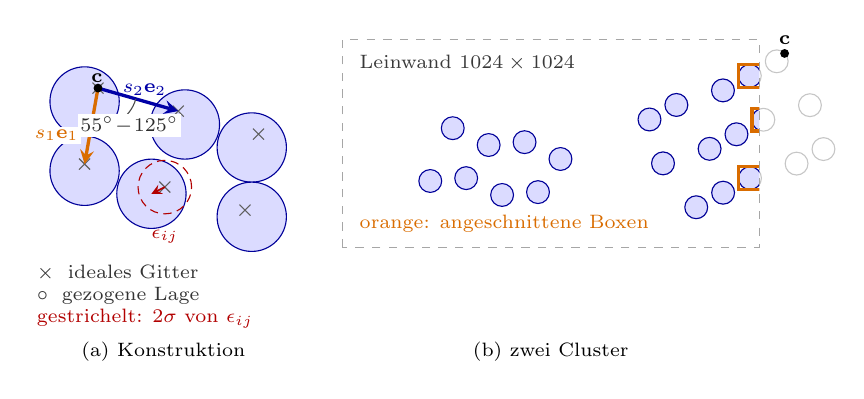
\begin{tikzpicture}[x=1cm,y=1cm]
% ================= (a) Gitterkonstruktion =================
\begin{scope}
  \pgfmathsetmacro{\cx}{0.62}
  \pgfmathsetmacro{\cy}{3.00}
  \pgfmathsetmacro{\ea}{-100}
  \pgfmathsetmacro{\eb}{-16}
  \pgfmathsetmacro{\sa}{0.98}
  \pgfmathsetmacro{\sb}{1.06}
  \pgfmathsetmacro{\rd}{0.44}
  % gezogene Lagen
  \foreach \i in {0,1}{\foreach \j in {0,1,2}{
    \pgfmathsetmacro{\ix}{\cx + \i*\sa*cos(\ea) + \j*\sb*cos(\eb)}
    \pgfmathsetmacro{\iy}{\cy + \i*\sa*sin(\ea) + \j*\sb*sin(\eb)}
    \pgfmathsetmacro{\jx}{0.085*(mod(7*\i+3*\j,5)-2)}
    \pgfmathsetmacro{\jy}{0.085*(mod(11*\i+5*\j,5)-2)}
    \fill[blue!14] ({\ix+\jx},{\iy+\jy}) circle (\rd);
    \draw[blue!60!black,thin] ({\ix+\jx},{\iy+\jy}) circle (\rd);}}
  % ideale Gitterpunkte darueber
  \foreach \i in {0,1}{\foreach \j in {0,1,2}{
    \pgfmathsetmacro{\ix}{\cx + \i*\sa*cos(\ea) + \j*\sb*cos(\eb)}
    \pgfmathsetmacro{\iy}{\cy + \i*\sa*sin(\ea) + \j*\sb*sin(\eb)}
    \draw[gray!75!black,thin] ({\ix-0.07},{\iy-0.07}) -- ({\ix+0.07},{\iy+0.07})
                              ({\ix-0.07},{\iy+0.07}) -- ({\ix+0.07},{\iy-0.07});}}
  % Basisvektoren
  \draw[->,>=stealth,very thick,orange!85!black] (\cx,\cy)
    -- ({\cx+\sa*cos(\ea)},{\cy+\sa*sin(\ea)});
  \node[font=\scriptsize,orange!85!black,anchor=east,inner sep=1pt,
        fill=white]
    at ({\cx+0.62*\sa*cos(\ea)-0.10},{\cy+0.62*\sa*sin(\ea)}) {$s_1\mathbf{e}_1$};
  \draw[->,>=stealth,very thick,blue!65!black] (\cx,\cy)
    -- ({\cx+\sb*cos(\eb)},{\cy+\sb*sin(\eb)});
  \node[font=\scriptsize,blue!65!black,anchor=south,inner sep=2pt]
    at ({\cx+0.58*\sb*cos(\eb)},{\cy+0.58*\sb*sin(\eb)}) {$s_2\mathbf{e}_2$};
  % eingeschlossener Winkel
  \draw[gray!60!black,thin] ({\cx+0.50*cos(\ea)},{\cy+0.50*sin(\ea)})
    arc[start angle=\ea, end angle=\eb, radius=0.50];
  \node[font=\scriptsize,gray!35!black,inner sep=1pt,fill=white]
    at ({\cx+0.62*cos(-50)},{\cy+0.62*sin(-50)}) {$55^\circ\!-\!125^\circ$};
  % Clusterzentrum
  \fill[black] (\cx,\cy) circle (1.6pt);
  \node[font=\scriptsize,anchor=south east,inner sep=1pt]
    at ({\cx+0.10},{\cy+0.03}) {$\mathbf{c}$};
  % Rauschen an einem Punkt hervorheben
  \pgfmathsetmacro{\hx}{\cx + \sa*cos(\ea) + \sb*cos(\eb)}
  \pgfmathsetmacro{\hy}{\cy + \sa*sin(\ea) + \sb*sin(\eb)}
  \pgfmathsetmacro{\hjx}{0.085*(mod(7*1+3*1,5)-2)}
  \pgfmathsetmacro{\hjy}{0.085*(mod(11*1+5*1,5)-2)}
  \draw[red!70!black,densely dashed,thin] (\hx,\hy) circle (0.34);
  \draw[->,>=stealth,red!70!black,semithick]
    (\hx,\hy) -- ({\hx+\hjx},{\hy+\hjy});
  \node[font=\scriptsize,red!70!black,anchor=north,inner sep=1pt]
    at ({\hx},{\hy-0.50}) {$\boldsymbol{\epsilon}_{ij}$};
  \node[font=\scriptsize,gray!40!black,anchor=north west,align=left]
    at (-0.28,0.88)
    {$\times$\; ideales Gitter\\$\circ$\; gezogene Lage\\
     \textcolor{red!70!black}{gestrichelt: $2\sigma$ von
     $\boldsymbol{\epsilon}_{ij}$}};
  \node[font=\scriptsize,anchor=north] at (1.45,-0.10) {(a) Konstruktion};
\end{scope}
% ================= (b) Leinwand =================
\begin{scope}[shift={(3.72,0)}]
  % Geisterkreise: das Gitter setzt sich ausserhalb der Leinwand fort
  \foreach \i in {0,1,2,3,4}{\foreach \j in {0,1,2}{
    \pgfmathsetmacro{\jx}{0.05*(mod(7*\i+3*\j,5)-2)}
    \pgfmathsetmacro{\jy}{0.05*(mod(11*\i+5*\j,5)-2)}
    \pgfmathsetmacro{\bx}{5.62 + \i*0.50*cos(-152) + \j*0.62*cos(-64) + \jx}
    \pgfmathsetmacro{\by}{3.44 + \i*0.50*sin(-152) + \j*0.62*sin(-64) + \jy}
    \draw[gray!45,thin] (\bx,\by) circle (0.145);}}
  \begin{scope}
    \clip (0,0.98) rectangle (5.30,3.62);
    \foreach \i in {0,1,2,3}{\foreach \j in {0,1}{
      \pgfmathsetmacro{\jx}{0.05*(mod(5*\i+2*\j,5)-2)}
      \pgfmathsetmacro{\jy}{0.05*(mod(13*\i+7*\j,5)-2)}
      \pgfmathsetmacro{\ax}{1.22 + \i*0.47*cos(-14) + \j*0.60*cos(72) + \jx}
      \pgfmathsetmacro{\ay}{1.92 + \i*0.47*sin(-14) + \j*0.60*sin(72) + \jy}
      \fill[blue!14] (\ax,\ay) circle (0.145);
      \draw[blue!60!black,thin] (\ax,\ay) circle (0.145);}}
    \foreach \i in {0,1,2,3,4}{\foreach \j in {0,1,2}{
      \pgfmathsetmacro{\jx}{0.05*(mod(7*\i+3*\j,5)-2)}
      \pgfmathsetmacro{\jy}{0.05*(mod(11*\i+5*\j,5)-2)}
      \pgfmathsetmacro{\bx}{5.62 + \i*0.50*cos(-152) + \j*0.62*cos(-64) + \jx}
      \pgfmathsetmacro{\by}{3.44 + \i*0.50*sin(-152) + \j*0.62*sin(-64) + \jy}
      \fill[blue!14] (\bx,\by) circle (0.145);
      \draw[blue!60!black,thin] (\bx,\by) circle (0.145);
      \ifdim\bx cm>5.02cm
        \draw[very thick,orange!85!black]
          ({\bx-0.145},{\by-0.145}) rectangle ({\bx+0.145},{\by+0.145});
      \fi}}
  \end{scope}
  \draw[dashed,gray!70] (0,0.98) rectangle (5.30,3.62);
  \node[font=\scriptsize,gray!45!black,anchor=north west] at (0.10,3.55)
       {Leinwand $1024 \times 1024$};
  \node[font=\scriptsize,orange!85!black,anchor=south west] at (0.10,1.04)
       {orange: angeschnittene Boxen};
  \fill[black] (5.62,3.44) circle (1.6pt);
  \node[font=\scriptsize,anchor=south,inner sep=3pt] at (5.62,3.44) {$\mathbf{c}$};
  \node[font=\scriptsize,anchor=north] at (2.65,-0.10) {(b) zwei Cluster};
\end{scope}
\end{tikzpicture}
\caption[Layoutmodell]{Das Layoutmodell aus Gleichung~\eqref{eq:layout}.
(a)~Konstruktion eines Clusters: Die Objektzentren liegen auf einem gescherten
Gitter mit den Basisrichtungen $\mathbf{e}_1$ und $\mathbf{e}_2$, deren
eingeschlossener Winkel zwischen $55^\circ$ und $125^\circ$ liegt; die
Gitterabstände liegen bei $s_1 \in [0{,}98;\,1{,}60]\,d_0$ und
$s_2 \in [0{,}98;\,1{,}85]\,d_0$. Auf jede ideale Gitterlage ($\times$) wirkt
zusätzlich das Rauschen $\boldsymbol{\epsilon}_{ij}$, sodass die gezogene Lage
($\circ$) um typischerweise $0{,}17\,d_0$ davon abweicht -- ohne diesen Term
entstünden sichtbar künstliche Reihen. (b)~Pro Bild werden ein bis drei solche
Cluster gezogen. Weil das Clusterzentrum $\mathbf{c}$ außerhalb der Leinwand
liegen darf, ragt ein Teil des Gitters (grau) über den Bildrand hinaus; von
diesen Objekten bleibt nur der sichtbare Teil, und ihre Boxen werden am
Bildrand abgeschnitten. In \code{test} sind 5,8\,\% der Labels angeschnitten.}
\label{abb:layout}
\end{figure}

\section{Sichtbarkeitsrechnung und Labelerzeugung}
\label{sec:sichtbarkeit}

Kein Copy-Paste-Generator darf Labels blind vergeben: Ein Objekt, das nach dem
Einfügen zu 95\,\% verdeckt ist, hat kein sinnvolles Label mehr. Für
\emph{jede} Instanz wird daher die exakte Sichtbarkeit berechnet. Grundlage ist
die Alpha-Kompositionsregel von \textcite{porter1984}: Wird Instanz $i$ von allen
später gemalten Schichten $j$ überlagert, so ist ihr sichtbarer Anteil
\begin{equation}
\alpha_i^{\text{sichtbar}} = \alpha_i \prod_{j > i} \big(1 - \alpha_j\big),
\qquad
v_i = \frac{\textstyle\sum \alpha_i^{\text{sichtbar}}}{\textstyle\sum \alpha_i},
\label{eq:sichtbarkeit}
\end{equation}
wobei das Produkt über \emph{alle} später gemalten Schichten läuft --
einschließlich anderer Profile, Rohrschäfte und Fremdkörper. Die Buchhaltung
läuft über die beschnittenen Alphafenster in Malreihenfolge, ist also exakt und
nicht approximiert.

Daraus folgen vier Regeln, die dieselben sind, nach denen \code{val} und
\code{test} annotiert wurden (Anforderung~A5): Ein Label wird verworfen, wenn die
Sichtbarkeit unter 30\,\% liegt (30\,801 Objekte, 17,8\,\% der gerenderten) --
unter 30\,\% sichtbarer Fläche wäre das Objekt auch für einen menschlichen
Annotator nicht mehr sicher identifizierbar, und \emph{kein} Label macht dieselbe
Bildstelle zum korrekten harten Negativ; wenn weniger als 15\,\% der Fläche im
Bild liegen (3\,846 Objekte); oder wenn die sichtbare Box unter 5\px{} fällt
(228 Objekte). Vergeben wird stets die \emph{modale} Box, also der sichtbare
Umriss. Insgesamt werden 34\,875 der 173\,100 gerenderten Instanzen verworfen
(20,1\,\%). Diese Zahl ist kein Verlust, sondern der Ertrag der Stufe: Sie
markiert genau jene Bildstellen, an denen ein naiver Generator ein falsches Label
gesetzt hätte.

\section{Der erzeugte Datensatz}
\label{sec:datensatz}

Es entstehen 6000 Bilder zu $1024\times1024$ Pixeln, davon 583 Negativbilder
(9,7\,\%), mit 136\,384 gelabelten Objekten (22,7 pro Bild) aus 173\,100
gerenderten Instanzen. Die mittlere Sichtbarkeit der gelabelten Objekte beträgt
90,0\,\%, 30,1\,\% von ihnen sind teilverdeckt. Der Objektdurchmesser liegt bei
p05/Median/p95 = 11,6/22,5/39,9\px, das Seitenverhältnis bei
p10/Median/p90 = 0,77/1,00/1,40.

Der wichtigste Qualitätsnachweis ist nicht der optische Eindruck, sondern der
Vergleich der erzeugten mit der gemessenen Statistik
(Tabelle~\ref{tab:kalibrierung}).

\begin{table}[htbp]
\centering
\caption[Kalibrierung gegen die Realmessung]{Kalibrierung des Layoutmodells
gegen die Realmessung ($n = 174$). Alle Abstände in Objektdurchmessern.}
\label{tab:kalibrierung}
\footnotesize
\begin{tabular}{@{}lccc@{}}
\toprule
\textbf{Kenngröße} & \textbf{real \code{val}} & \textbf{real \code{test}} &
\textbf{synthetisch (Ist)} \\
\midrule
NN-Abstand p10 / Median / p90 & 0,86 / 1,09 / 1,78 &
0,83 / 1,24 / 2,51 & \textbf{0,84 / 1,17 / 1,87} \\
berührt den NN ($< 1{,}2\,\Oe$) & 61,4\,\% & 46,5\,\% & \textbf{53,6\,\%} \\
Nachbarn innerhalb $5\,\Oe$ (Median) & 10 & 10 & \textbf{13} \\
Größenverhältnis zum NN (Median) & 1,05 & 1,05 &
\textbf{1,05} (per Konstruktion) \\
\bottomrule
\end{tabular}
\end{table}

Die synthetische Verteilung liegt bei allen vier Kenngrößen zwischen oder nahe
bei den beiden realen Messungen. Die einzige systematische Abweichung ist die
Nachbarzahl: Die synthetischen Cluster sind dichter (13 statt 10 Nachbarn
innerhalb $5\,\Oe$, im Maximum 61 statt 20). Das ist bewusst so belassen -- eine
höhere Dichte im Training ist eine Robustheitsreserve, weil sie den Detektor auf
schwierigere Szenen vorbereitet als die, die er zur Inferenzzeit vorfindet. Die
umgekehrte Abweichung wäre gefährlich gewesen.

\section{Nachweis der Anforderungen}
\label{sec:nachweis}

Anforderung~\textbf{A1} ist erfüllt, weil die Box nach jeder
Instanztransformation aus der transformierten Alphamaske neu bestimmt wird und
die boxverfälschenden Operationen zur Trainingszeit auf~0 stehen.
\textbf{A2}: Objektgrößen 12--44\px{} aus der Realmessung, Leinwandgröße gleich
der Trainingsauflösung. \textbf{A3}: Maßstabskopplung, Schaft hinter jeder
Stirnfläche, parallele Schaftrichtung, Tiefenmodell 75/25, volle Rotation.
\textbf{A4}: S1 Alphamaske und Kantenweichzeichnung, S2 partieller Farbangleich,
S3 flächentreue Skalierung und Unschärfeangleich, S4 lokal geschätzter
Rauschangleich, S5 JPEG-Requantisierung, S6 Schlagschatten und physikalische
Verdeckung. \textbf{A5}: modale Boxen und dieselben Verwerfungsregeln wie bei der
Handannotation -- allerdings nur \emph{annähernd}, wie
Abschnitt~\ref{sec:boxversatz} zeigt: Die Generatorboxen folgen der
$\alpha > 0{,}5$-Kontur und fallen damit um 1,2 bis 2,5\px{} kleiner aus als die
Handannotation. \textbf{A6}: Tabelle~\ref{tab:parameter} mit Sollbereich und
gemessenem Ist-Anteil je Transformation, sieben Werte ausdrücklich als Annahme
gekennzeichnet.

Die Anforderungen sind damit \emph{formal} erfüllt. Das sagt nichts darüber aus,
ob die einzelnen Maßnahmen \emph{wirken} -- die Erfüllung einer
Entwurfsanforderung ist kein empirischer Nachweis. Diese Unterscheidung wird in
Kapitel~\ref{kap:auswertung} durch die Messung des Sim-to-Real-Abstands und die
Okklusionsablation adressiert und in Abschnitt~\ref{sec:tragend} bilanziert.
